\chapter{Исследование работы баз данных}


\section{Подготовка тестовых данных}

Для тестирования будут использованы три различных графа, взятые из коллекции больших сетевых данных Стэнфорда — https://snap.stanford.edu/data/:

\begin{itemize}
    \item CollegeMsg temporal network (далее COL) — ориентированный граф, содержащий 1899 вершин и 59835 ребер из которых 20296 являются уникальными. Этот набор данных состоит из личных сообщений, отправленных пользователями в социальной сети. Узлы представляют собой пользователей, а рёбра — факт отправки личного сообщения от одного пользователя другому. Особенностью графа является большое количество кратных рёбер, а именно 39539;
    \item Gnutella peer-to-peer network, 5 Aug 2002 (далее GNU) – ориентированный граф, содержащий 8846 вершин и 31839 ребер. Этот набор данных представляет собой снимок одноранговой файлообменной сети Gnutella за 9 августа 2002 года. Узлы представляют собой хосты в топологии сети Gnutella, а ребра - соединения между хостами Gnutella. Особенностью графа является низкий средний коэффициент кластеризации – 0.0072;
    \item Social circles: Facebook (далее FB) — ориентированный граф, содержащий 3483 вершины и 50865 ребер. Этот набор данных состоит из списка отправленных заявок на добавления в друзья на Facebook. Узлы представляют собой пользователей, а рёбра — факт отправки запроса на добавления в друзья. Особенностью графа является высокий средний коэффициент кластеризации – 0.6055.
\end{itemize}


\section{Исследование способов хранения графовых данных}

Для хранения графовых данных в PostgreSQL потребуются три таблицы:

\begin{itemize}
    \item entity — описывает сущности, которые могут являться объектом или субъектом отношения. Хранит уникальный идентификатор сущности, её название и метаданные;
    \item predicate — описывает тип отношения. Хранит уникальный идентификатор отношения и его название;
    \item triple — содержит информацию об объекте, субъекте, типе отношения между ними и метаданные этого отношения.
\end{itemize}

\begin{figure}[ht!]
    \center
    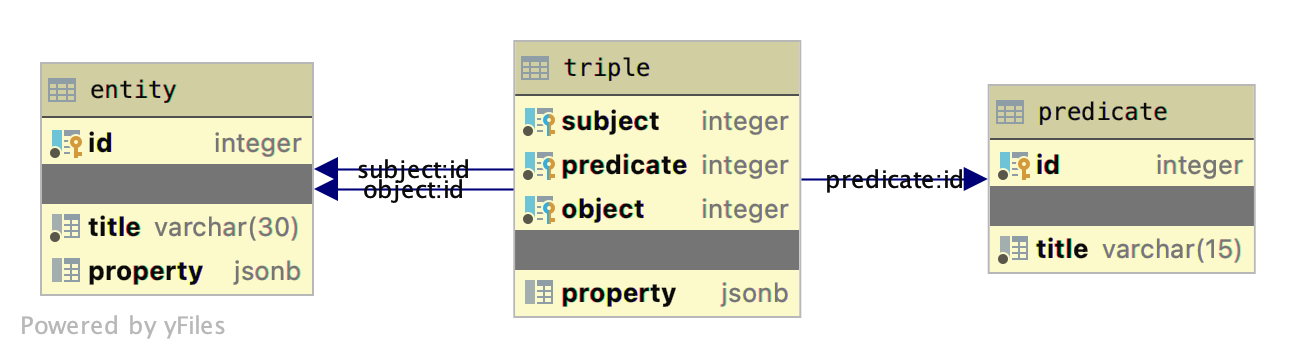
\includegraphics [scale=0.35] {my_folder/myimg//8}
    \caption{Диаграмма структуры базы данных PostgreSQL для хранения графа}
\end{figure}

Для хранения графовых данных в Neo4j не требуется никаких дополнительных настроек.

Для хранения графовых данных в ArangoDB необходимо создать коллекцию типа “Document” для хранения сущностей и коллекцию типа “Edges” для
хранения отношений, после чего необходимо создать граф, с настройками, как указано на рис.4.2.

\begin{figure}[ht!]
    \center
    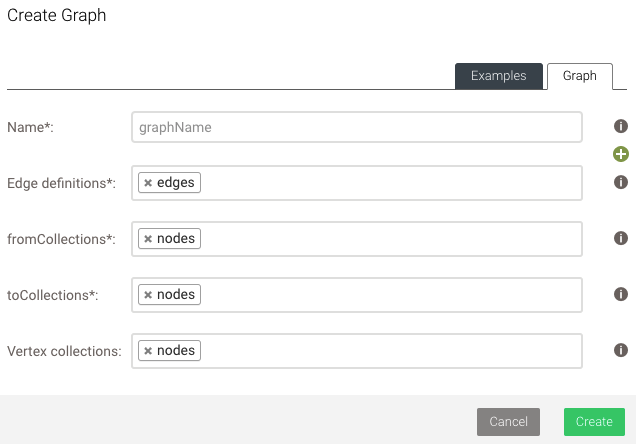
\includegraphics [scale=0.5] {my_folder/myimg//9}
    \caption{Создание графа в ArangoDB на основе двух коллекций}
\end{figure}

От структуры хранения графовых данных напрямую зависит количество памяти, которое понадобится базе данных для хранения загруженного графа.
Результаты замеров использованной памяти для каждого из тестовых графов приведены в таблице 4.1.

\begin{table} [htbp]
    \centering\small
    \caption{Количество памяти, необходимое базе данных для хранения графа}
    \begin{tabular}{|l|l|p{3cm}|}
        \hline
        База данных & Граф & Использованная память \\ \hline
        PostgreSQL  & COL  & 10 Мб                 \\ \hline
        PostgreSQL  & GNU  & 11 Мб                 \\ \hline
        PostgreSQL  & FB   & 12 Мб                 \\ \hline
        Neo4j       & COL  & 239 Мб                \\ \hline
        Neo4j       & GNU  & 396 Мб                \\ \hline
        Neo4j       & FB   & 427 Мб                \\ \hline
        ArangoDB    & COL  & 44 Мб                 \\ \hline
        ArangoDB    & GNU  & 66 Мб                 \\ \hline
        ArangoDB    & FB   & 53 Мб                 \\ \hline
    \end{tabular}
    \normalsize
\end{table}

Из таблицы 4.1 можно сделать вывод, что после занесении информации о графе в базу данных Neo4j, её размер превышает размер базы данных
PostgreSQL примерно в 30 раз и размер базы данных ArangoDB примерно в 6 раз.


\section{Исследование функциональности и производительности языка запросов при вставке данных}

Результаты замеров времени поочередной вставки записей об отношениях в базы PostgreSQL и ArangoDB приведены в таблице 4.2.

\begin{table} [htbp]
    \centering\small
    \caption{Время поочередной вставки записей об отношениях в базы данных}
    \begin{tabular}{|p{3cm}|p{1cm}|p{2cm}|p{2cm}|p{2cm}|p{2cm}|p{2cm}|}
        \hline
        База данных & Граф & Среднее время & Стандартное отклонение & 95-ый процентиль & 98-ой процентиль & Суммарное время \\ \hline
        PostgreSQL  & COL  & 2.44 мс       & 0.69 мс                & 3.07 мс          & 3.53 мс          & 50 сек          \\ \hline
        PostgreSQL  & GNU  & 2.65 мс       & 0.83 мс                & 3.56 мс          & 4.07 мс          & 85 сек          \\ \hline
        PostgreSQL  & FB   & 2.72 мс       & 1.07 мс                & 3.77 мс          & 4.46 мс          & 139 сек         \\ \hline
        ArangoDB    & COL  & 2.46 мс       & 0.98 мс                & 3.69 мс          & 4.73 мс          & 50 сек          \\ \hline
        ArangoDB    & GNU  & 2.47 мс       & 0.91 мс                & 3.61 мс          & 4.69 мс          & 78 сек          \\ \hline
        ArangoDB    & FB   & 2.40 мс       & 0.86 мс                & 3.73 мс          & 4.61 мс          & 122 сек         \\ \hline
    \end{tabular}
    \normalsize
\end{table}

По таблице 4.2 видно, что операции поочередной вставки записей об отношениях в базы PostgreSQL и ArangoDB незначительно отличаются друг от
друга по времени выполнения. База данных Neo4j в отличие от других не оптимизирована под единичную вставку, но оптимизирована под
множественную вставку данных. Результаты замеров суммарного времени вставки записей об отношениях в базу данных Neo4j приведены в таблице 4.3.

\begin{table} [htbp]
    \centering\small
    \caption{Время множественной вставки записей об отношениях в базу данных Neo4j}
    \begin{tabular}{|l|l|l|}
        \hline
        База данных & Граф & Суммарное время \\ \hline
        Neo4j       & COL  & 30.46 сек       \\ \hline
        Neo4j       & GNU  & 46.15 сек       \\ \hline
        Neo4j       & FB   & 58.35 сек       \\ \hline
    \end{tabular}
    \normalsize
\end{table}

Сравнивая результаты затраченного времени на вставку всех записей об отношениях из таблицы 4.2 и таблицы 4.3 можно сделать вывод, что база
данных Neo4j примерно в 2 раза быстрее справляется с поставленной задачей за счёт оптимизации множественной вставки данных.


\section{Исследование функциональности и производительности языка запросов при извлечении данных}

Структура хранения графовой информации подразумевает возможность наличие у сущности неограниченного количества атрибутов. Например для
сущности человек, могут существовать атрибуты: имя, дата рождения, пол, гендер и так далее. Результаты замеров времени при извлечении
данных о сущностях на основе атрибутов представлены в таблице 4.4.

\begin{table} [htbp]
    \centering\small
    \caption{Время извлечение данных на основе атрибутов сущности}
    \begin{tabular}{|p{3cm}|p{1cm}|p{2cm}|p{2cm}|p{2cm}|p{2cm}|}
        \hline
        База данных & Граф & Среднее время & Стандартное отклонение & 95-ый процентиль & 98-ой процентиль \\ \hline
        PostgreSQL  & COL  & 16,84 мс      & 8,91 мс                & 23,37 мс         & 29,67 мс         \\ \hline
        PostgreSQL  & GNU  & 26,08 мс      & 10,44 мс               & 36,98 мс         & 42,78 мс         \\ \hline
        PostgreSQL  & FB   & 36,21 мс      & 10,98 мс               & 50,82 мс         & 54,56 мс         \\ \hline
        Neo4j       & COL  & 29.23 мс      & 15.12 мс               & 51.71 мс         & 72.10 мс         \\ \hline
        Neo4j       & GNU  & 71.53 мс      & 29.36 мс               & 111.25 мс        & 135.28 мс        \\ \hline
        Neo4j       & FB   & 37.12 мс      & 24.89 мс               & 57.86 мс         & 86.05 мс         \\ \hline
        ArangoDB    & COL  & 13.54 мс      & 4.32 мс                & 22.14 мс         & 24.47 мс         \\ \hline
        ArangoDB    & GNU  & 56.41 мс      & 9.97 мс                & 67.73 мс         & 81.72 мс         \\ \hline
        ArangoDB    & FB   & 23.41 мс      & 4.93 мс                & 31.38 мс         & 38.22 мс         \\ \hline
    \end{tabular}
    \normalsize
\end{table}

Также структура графовой информации подразумевает возможность наличия у отношения неограниченного количества атрибутов. Например для
отношения “сыграл в фильме” могут существовать атрибуты: роль, количество времени в кадре и так далее. Результаты замеров времени при
извлечении данных об отношениях на основе атрибутов представлены в таблице 4.5.

\begin{table} [htbp]
    \centering\small
    \caption{Время извлечение данных на основе атрибутов отношения}
    \begin{tabular}{|p{3cm}|p{1cm}|p{2cm}|p{2cm}|p{2cm}|p{2cm}|}
        \hline
        База данных & Граф & Среднее время & Стандартное отклонение & 95-ый процентиль & 98-ой процентиль \\ \hline
        PostgreSQL  & COL  & 70.78 мс      & 38.27 мс               & 109.79 мс        & 126.06 мс        \\ \hline
        PostgreSQL  & GNU  & 107.57 мс     & 51.01 мс               & 156.08 мс        & 187.07 мс        \\ \hline
        PostgreSQL  & FB   & 153.91 мс     & 47.74 мс               & 217.96 мс        & 251.98 мс        \\ \hline
        Neo4j       & COL  & 148.87 мс     & 58.64 мс               & 222.54 мс        & 253.59 мс        \\ \hline
        Neo4j       & GNU  & 207.4 мс      & 39.38 мс               & 292.25 мс        & 326.44 мс        \\ \hline
        Neo4j       & FB   & 313.45 мс     & 72.98 мс               & 417.73 мс        & 490.48 мс        \\ \hline
        ArangoDB    & СOL  & 153.81 мс     & 9.32 мс                & 167.09 мс        & 186.26 мс        \\ \hline
        ArangoDB    & GNU  & 238.35 мс     & 12 мс                  & 255.77 мс        & 276.04 мс        \\ \hline
        ArangoDB    & FB   & 374.64 мс     & 17.5 мс                & 399.9 мс         & 425.61 мс        \\ \hline
    \end{tabular}
    \normalsize
\end{table}

Из таблиц 4.4 и 4.5 можно сделать вывод, что извлечение данных на основе атрибутов быстрее всего происходит происходит из базы PostgreSQL,
ArangoDB работает в среднем в 1.5 раз дольше, а Neo4j в отстаёт от PostgreSQL в среднем в 2 раза. Такие различия между реляционной и
нереляционными базами данных обоснованы способом хранения информации. С помощью правильной декомпозиции графовой структуры данных на три
таблицы удалось обеспечить высокую скорость работы с любыми типами атрибутов.

Помимо извлечения данных на основе атрибутов, не менее частой задачей является извлечение данных на основе графовых алгоритмов. Чаще всего
применяются следующие алгоритмы: поиск кратчайшего пути, поиск ближайших соседей, ранжирование Пейджа, определение степени влиятельности.
Результаты замеров времени при извлечении данных на основе алгоритма поиска кратчайшего пути представлены в таблице 4.6.

\begin{table} [htbp]
    \centering\small
    \caption{Время извлечение данных на основе алгоритма поиска кратчайшего пути}
    \begin{tabular}{|p{3cm}|p{1cm}|p{2cm}|p{2cm}|p{2cm}|p{2cm}|}
        \hline
        База данных & Граф & Среднее время & Стандартное отклонение & 95-ый процентиль & 98-ой процентиль \\ \hline
        PostgreSQL  & COL  & 85.23 мс      & 21.15 мс               & 119.53 мс        & 124.49 мс        \\ \hline
        PostgreSQL  & GNU  & 130.41 мс     & 25.77 мс               & 170.42 мс        & 223.52 мс        \\ \hline
        PostgreSQL  & FB   & 215.04 мс     & 51.87 мс               & 303.44 мс        & 319.79 мс        \\ \hline
        Neo4j       & COL  & 8.99 мс       & 4.95 мс                & 11.91 мс         & 14.38 мс         \\ \hline
        Neo4j       & GNU  & 14.18 мс      & 6.21 мс                & 20.56 мс         & 26.99 мс         \\ \hline
        Neo4j       & FB   & 12.01 мс      & 8.18 мс                & 17.14 мс         & 19.58 мс         \\ \hline
        ArangoDB    & COL  & 2.69 мс       & 0.62 мс                & 3.53 мс          & 3.92 мс          \\ \hline
        ArangoDB    & GNU  & 2.99 мс       & 0.72 мс                & 4.16 мс          & 4.66 мс          \\ \hline
        ArangoDB    & FB   & 3.72 мс       & 1.41 мс                & 6.18 мс          & 7.16 мс          \\ \hline
    \end{tabular}
    \normalsize
\end{table}

По таблице 4.6 видно, что быстрее всего с задачей поиска кратчайшего пути справляется база данных ArangoDB, примерно в 3.5 раз дольше этот
же алгоритм работает в базе данных Neo4j и примерно в 30 раз дольше с аналогичной задачей справляется сервис, основанный на базе данных
PostgreSQL. Такой результат вызван отсутствием поддержки графовых алгоритмов в PostgreSQL, вследствии чего задачей занимается сервисный
слой, которому необходимо предварительно извлечь все данные для построения графа.

Результаты замеров времени при извлечении данных на основе алгоритма поиска ближайших соседей представлены в таблице 4.7.

\begin{table} [htbp]
    \centering\small
    \caption{Время извлечение данных на основе алгоритма поиска ближайших соседей}
    \begin{tabular}{|p{3cm}|p{1cm}|p{2cm}|p{2cm}|p{2cm}|p{2cm}|}
        \hline
        База данных & Граф & Среднее время & Стандартное отклонение & 95-ый процентиль & 98-ой процентиль \\ \hline
        PostgreSQL  & COL  & 144.25 сек    & 63.46 сек              & 193.83 сек       & 217.32 сек       \\ \hline
        PostgreSQL  & GNU  & -             & -                      & -                & -                \\ \hline
        PostgreSQL  & FB   & -             & -                      & -                & -                \\ \hline
        Neo4j       & COL  & 6.33 сек      & 5.98 сек               & 12.15 сек        & 16.49 сек        \\ \hline
        Neo4j       & GNU  & 17.82 сек     & 7.11 сек               & 22.51 сек        & 27.98 сек        \\ \hline
        Neo4j       & FB   & 15.79 сек     & 7.83 сек               & 23.85 сек        & 26.54 сек        \\ \hline
        ArangoDB    & COL  & 0.88 сек      & 0.25 сек               & 1.29 сек         & 1.43 сек         \\ \hline
        ArangoDB    & GNU  & 1.51 сек      & 0.61 сек               & 2.41 сек         & 2.95 сек         \\ \hline
        ArangoDB    & FB   & 1.35 сек      & 0.89 сек               & 2.44 сек         & 3.56 сек         \\ \hline
    \end{tabular}
    \normalsize
\end{table}

Из таблицы 4.7 видно, что лучше всего с задачей поиска ближайших соседей справляется база данных ArangoDB, примерно в 10 раз больше времени
требуется Neo4j для решения аналогичной задачи, а PostgreSQL даже при наличии сервисного слоя работает в сотни раз дольше на самом маленьком
из тестовых графов, а на двух больших графах и вовсе не смогла справиться с поставленной задачей ввиду нехватки память для вычислений,
выделенной в рамках исследования.


\section{Итоги исследований}

После правильной адаптации для хранения графовых структур реляционная база данных PostgreSQL использует намного меньше дискового пространства
и способна обеспечить конкурентоспособную вставку графовых данных на уровне нереляционных баз данных. Однако проблема отсутствия поддержки
графовых алгоритмов обработки для извлечения данных не способна быть эффективно решена посредством добавления сервисного слоя. Это связано
с тем, что для правильной работы сервисного слоя необходимо получить из базы всю имеющуюся информацию и обработать её повторно для построения
графовой структуры на сервисе. Такое решение способно поддерживать небольшие графовые структуры, но оказывается совершенно неработоспособным
при увеличении количества данных ввиду ограниченности оперативной памяти сервиса.

Графовая база данных Neo4j способна удовлетворить любые потребности в хранении и обработке графовых структур за счёт своей реализации и языка
Cypher, но требует ощутимо больше дисковой памяти для хранения информации. Наличие поддержки и оптимизации для множественной вставки графовых
данных выделяет эту базу данных на фоне конкурентов, но оптимизации встроенных механизмов отбора и извлечения данных, а также графовых
алгоритмов зачастую недостаточно для уверенной победы над конкурентами в вопросах времени выполнения. При этом база данных Neo4j способна
поддерживать графовые структуры данных очень большого объёма и предоставляет исчерпывающее количество инструментов для продуктивного
взаимодействия с графовыми данными, среди которых можно выделить инструменты графо-нативного машинного обучения и мощное браузерное
приложения для администрирования и управления данными.

Мультимодельная база данных ArangoDB при решении задач хранения графовых структур использует лучшее от документоориентированного и графового
подхода к хранению данных. За счёт документоориентированного подхода, графовые данные хранимые в ArangoDB занимают незначительно больше места,
чем в реляционной базе данных, а извлечение данных на основе атрибутов происходит быстро. За счёт графового подхода к обработке информации
ArangoDB предоставляет мощные и быстрые инструменты языка AQL для извлечения данных на основе графовых алгоритмов. Но в отличие от Neo4j эта
база данных не имеет развитого инструментария для извлечения всех возможностей графовых данных, что делает её менее привлекательной для
проектов, нуждающихся в оптимизации для большого количества данных и наличия продвинутых графовых алгоритмов и встроенного машинного обучения.

%% Вспомогательные команды - Additional commands
%
%\newpage % принудительное начало с новой страницы, использовать только в конце раздела
%\clearpage % осуществляется пакетом <<placeins>> в пределах секций
%\newpage\leavevmode\thispagestyle{empty}\newpage % 100 % начало новой страницы